\subsection{Strong Interactions}
\label{sec:Intro_QCD}

\begin{figure}[htb]
  \begin{center}
    {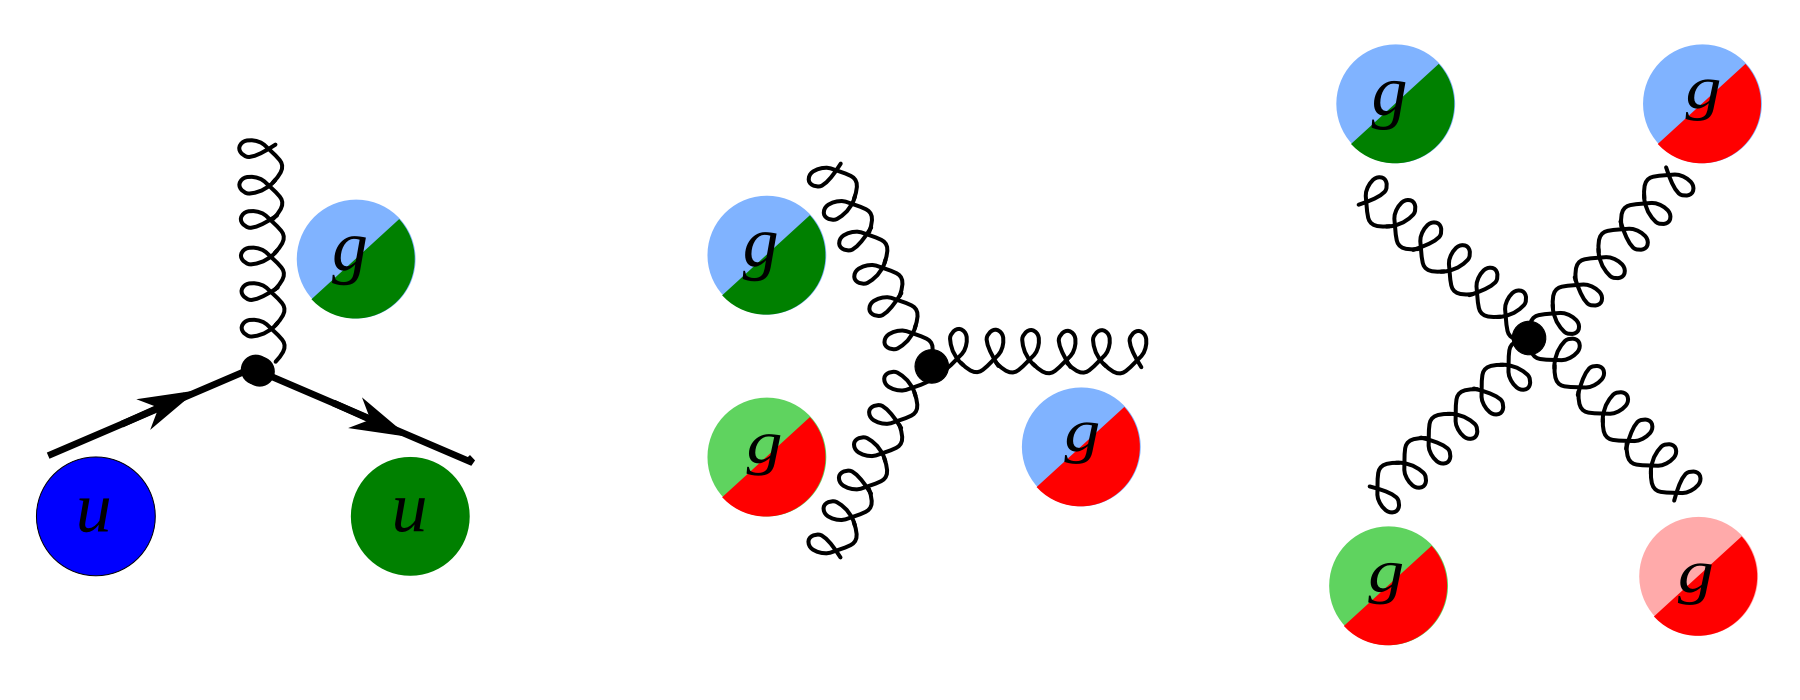
\includegraphics[width=0.90\textwidth]{../figs/Intro/feynmStrong.png}}
    \caption{Strong interations}
    \label{fig:feynmStrong}
  \end{center}
\end{figure}

 %  Again, I do not see a connective narrative. Paragraphs are sets of loosely connected sentences, the section is a set of loosely connected paragraphs. Needs imporvement.
% Somewhat reverse flow of ideas, example:
% > There are eight types of gluons corresponding to different color-anticolor combinations.
% > Gluons are spin-one massless electrically neutral particles.
% First, you should say what gluons ARE, and then you can say what types of gluons exist.
% > Gluons possess color charges, therefore, they can self-interact.
% The emphasis of this statement is that gluons possess color charges, which is odd because you already mentioned it some number of times above (which adds to the feeling of reverse flow).
% Instead, the emphasis of the sentence should be that they can self-inteact.
% Some incorrect information, for example:
% "it becomes larger as the distance becomes smaller” about the coupling constant: it becomes smaller at smaller distances, larger at larger distances.

The third fundamental force after the electromagnetic and weak ones is the strong force. The strong force is responsible for glueing protons and neutrons together in the nuclea as well as for forming protons and neutrons themselves. The strong interactions are performed by exchanging gluons which are spin-one massless electrically neutral particles.  \\

The elementary strong processes are shown in Fig. \ref{fig:feynmStrong}. There are three elementary processes: qqg, ggg and gggg, all are involving particles with color charges. Thus, gluons couple to quarks and self-couple. Color charges must be conserved at each elementary process of the strong interaction. And because quarks can possess three colors, there are eight types of gluons to cover all possible color exchanges. \\

The coupling constant of the strong interaction depends on a distance between interacting particles: it becomes larger as the distance becomes larger. This property leads to two consequences specific to the strong force: the confinement and the asymptotic freedom.\\

The confinement is the property of quarks to always stay in the colorly neutral combinations (hadrons), it forbids the existence of free quarks. A combination becomes colorly neutral when there is the same amount of color and anticolor or if there is the same amount of each of the three colors.  There are two types of hadros: mesons (comprised of a quark and antiquarks with the opposite color charges) and baryons (comprised of three quarks: a red, a green and a blue one). The widely known particles a proton and a neutron are baryons.\\

The asymptotic freedom means that when quarks are very close to each other they almost do not interact with each other and therefore they are free. When the distance between quarks is low which corresponds to high energy, and thus the coupling constant $1/\alpha_s \ll 1$ is low, the strong interactions can be described by a perturbative quantum field theory which is called quantum chromodynamics (QCD).\\

The W$\gamma$ process being measured in this dissertation is not intended to test QCD, but a good understanding of QCD is essential for performing this measurement. First of all, QCD describes the dynamics of quarks and gluons within colliding protons and predicts probabilities of one or another quark-antiquark pair to annihilate. Secondly, the QCD corrections to the Feynman diagrams of the process are large and has to be taken into account in producing simulation. Possible QCD correction include quark-gluon loops at any of three quark lines as well as exchanges of gluons between different quark lines.\\
 
